\definecolor{c333333}{RGB}{51,51,51}
\definecolor{c2c2b31}{RGB}{44,43,49}
\definecolor{c1c1b22}{RGB}{28,27,34}
\definecolor{c2e2e38}{RGB}{46,46,56}
\definecolor{c384c5a}{RGB}{56,76,90}
\definecolor{cbebebe}{RGB}{190,190,190}
\definecolor{c699ad7}{RGB}{105,154,215}
\definecolor{c7ebae4}{RGB}{126,186,228}
\definecolor{c859fd5}{RGB}{133,159,213}
\definecolor{c7fecff}{RGB}{127,236,255}
\definecolor{cc1f6ff}{RGB}{193,246,255}


\def \globalscale {1.000000}
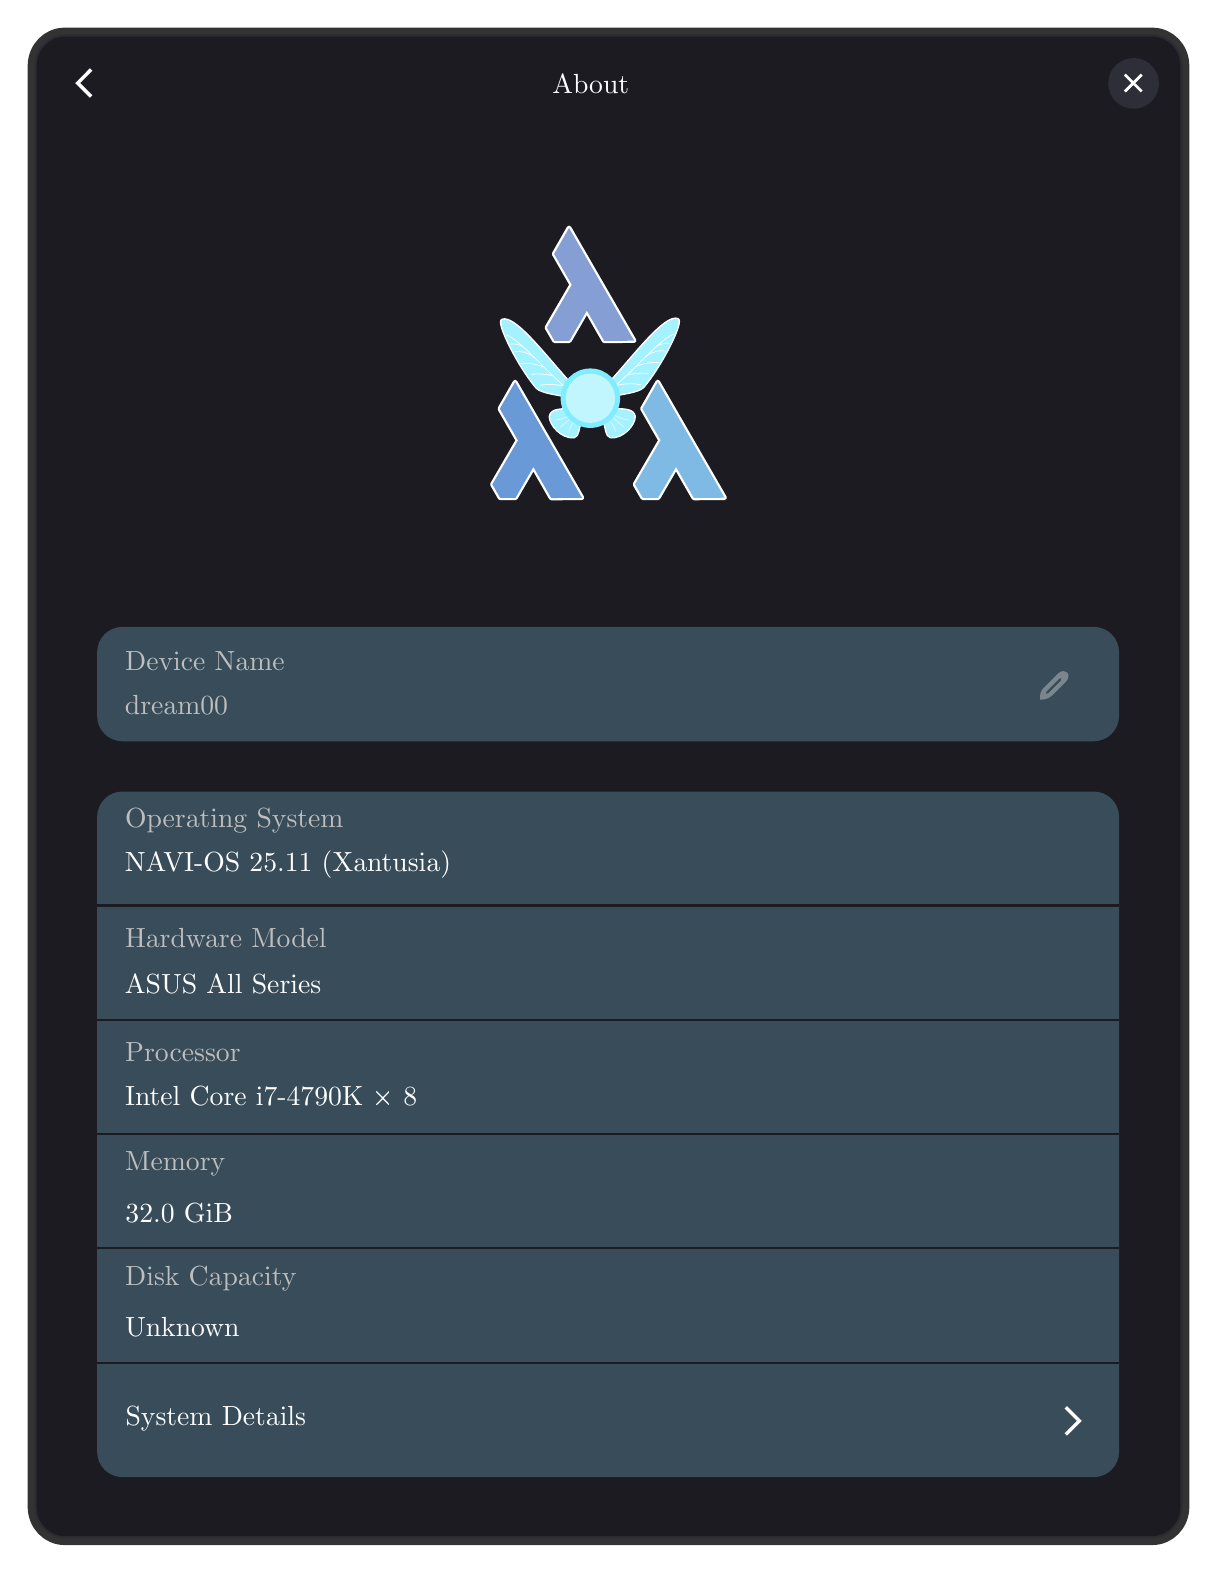
\begin{tikzpicture}[y=1cm, x=1cm, yscale=\globalscale,xscale=\globalscale, every node/.append style={scale=\globalscale}, inner sep=0pt, outer sep=0pt]
  \begin{scope}[shift={(-1.2269, 4.1128)}]
    \path[draw=c333333,line cap=round,line join=round,line width=0.2cm] (2.0851, 15.446) -- (15.8977, 15.446).. controls (16.1028, 15.446) and (16.2679, 15.2742) .. (16.2679, 15.0607) -- (16.2679, -3.2395).. controls (16.2679, -3.453) and (16.1028, -3.6248) .. (15.8977, -3.6248) -- (2.0851, -3.6248).. controls (1.88, -3.6248) and (1.7149, -3.453) .. (1.7149, -3.2395) -- (1.7149, 15.0607).. controls (1.7149, 15.2742) and (1.88, 15.446) .. (2.0851, 15.446) -- cycle;



    \path[draw=c2c2b31,fill=c1c1b22,line width=0.0265cm] (2.0851, 15.446) -- (15.8977, 15.446).. controls (16.1028, 15.446) and (16.2679, 15.2742) .. (16.2679, 15.0607) -- (16.2679, -3.2395).. controls (16.2679, -3.453) and (16.1028, -3.6248) .. (15.8977, -3.6248) -- (2.0851, -3.6248).. controls (1.88, -3.6248) and (1.7149, -3.453) .. (1.7149, -3.2395) -- (1.7149, 15.0607).. controls (1.7149, 15.2742) and (1.88, 15.446) .. (2.0851, 15.446) -- cycle;



    \path[fill=c2e2e38,line width=0.0265cm] (15.9814, 14.8379)arc(0.0:90.0001:0.3218 and -0.3218)arc(90.0:180.0:0.3218 and -0.3218)arc(180.0:270.0:0.3218 and -0.3218)arc(-90.00009999999997:0.0:0.3218 and -0.3218) -- cycle;



    \node[text=white,anchor=south west,line width=0.0364cm] (text1) at (8.278, 14.7067){About};



    \path[fill=white,line width=0.0364cm] (15.7757, 14.9371) -- (15.6812, 14.8422) -- (15.7757, 14.7477) -- (15.7511, 14.7227) -- (15.6562, 14.8176) -- (15.5613, 14.7227) -- (15.5369, 14.7477) -- (15.6312, 14.8422) -- (15.5369, 14.9371) -- (15.5613, 14.9621) -- (15.6562, 14.8672) -- (15.7511, 14.9621) -- cycle;



    \path[fill=white,line width=0.0364cm] (2.4058, 14.6556) -- (2.2189, 14.8427) -- (2.4058, 15.0299) -- (2.4364, 14.9992) -- (2.2802, 14.8427) -- (2.4364, 14.6862) -- cycle;



    \path[fill=c384c5a,line width=0.0262cm] (2.8197, 7.9362) -- (15.1527, 7.9362).. controls (15.3316, 7.9362) and (15.4756, 7.7922) .. (15.4756, 7.6133) -- (15.4756, 6.8056).. controls (15.4756, 6.6268) and (15.3316, 6.4828) .. (15.1527, 6.4828) -- (2.8197, 6.4828).. controls (2.6408, 6.4828) and (2.4968, 6.6268) .. (2.4968, 6.8056) -- (2.4968, 7.6133).. controls (2.4968, 7.7922) and (2.6408, 7.9362) .. (2.8197, 7.9362) -- cycle;



    \path[fill=c384c5a,line width=0.0262cm] (2.8197, 5.8448) -- (15.1527, 5.8448).. controls (15.3316, 5.8448) and (15.4756, 5.7008) .. (15.4756, 5.5219) -- (15.4756, -2.539).. controls (15.4756, -2.7179) and (15.3316, -2.8619) .. (15.1527, -2.8619) -- (2.8197, -2.8619).. controls (2.6408, -2.8619) and (2.4968, -2.7179) .. (2.4968, -2.539) -- (2.4968, 5.5219).. controls (2.4968, 5.7008) and (2.6408, 5.8448) .. (2.8197, 5.8448) -- cycle;



    \node[text=white,anchor=south west,line width=0.0364cm] (text1-9-2-6) at (2.8578, -2.2738){System Details};



    \node[text=cbebebe,anchor=south west,line width=0.0364cm] (text1-9-46-0) at (2.8501, 6.8209){dream00};



    \node[text=cbebebe,anchor=south west,line width=0.0364cm] (text1-9-46-7-4) at (2.8532, -0.4977){Disk Capacity};



    \node[text=cbebebe,anchor=south west,line width=0.0364cm] (text1-9-46-7-8-26) at (2.8539, 0.959){Memory};



    \node[text=cbebebe,anchor=south west,line width=0.0364cm] (text1-9-46-7-8-2-5) at (2.854, 2.4117){Processor};



    \node[text=cbebebe,anchor=south west,line width=0.0364cm] (text1-9-46-7-8-2-0-9) at (2.8526, 3.8609){Hardware Model};



    \node[text=cbebebe,anchor=south west,line width=0.0364cm] (text1-9-46-7-8-2-6-7) at (2.8511, 5.3205){Operating System};



    \node[text=cbebebe,anchor=south west,line width=0.0364cm] (text1-9-46-7-8-2-8-8) at (2.8528, 7.3817){Device Name};



    \node[text=white,anchor=south west,line width=0.0364cm] (text1-9-9) at (2.8521, 1.8236){Intel Core i7-4790K × 8};



    \path[fill=white,line width=0.0428cm] (14.8148, -2.3346) -- (15.0016, -2.1475) -- (14.8148, -1.9604) -- (14.7841, -1.991) -- (14.9404, -2.1475) -- (14.7841, -2.304) -- cycle;



    \node[text=white,anchor=south west,line width=0.0364cm] (text1-9-8-2) at (2.8573, 0.3777){32.0 GiB};



    \node[text=white,anchor=south west,line width=0.0364cm] (text1-9-4-6) at (2.8518, -1.0811){Unknown};



    \node[text=white,anchor=south west,line width=0.0364cm] (text1-9-1-32) at (2.8508, 3.2842){ASUS All Series};



    \node[text=white,anchor=south west,line width=0.0364cm] (text1-9-1-3-5) at (2.8501, 4.7381){NAVI-OS 25.11 (Xantusia)};



    \path[fill=cbebebe,opacity=0.5008,line width=0.0303cm] (14.7683, 7.3749).. controls (14.7451, 7.3742) and (14.7198, 7.3632) .. (14.6994, 7.3428) -- (14.5197, 7.1632).. controls (14.4502, 7.0936) and (14.4743, 7.0131) .. (14.4743, 7.0131).. controls (14.4743, 7.0131) and (14.5625, 7.0029) .. (14.6213, 7.0617) -- (14.8009, 7.2413).. controls (14.8371, 7.2775) and (14.8437, 7.3293) .. (14.8155, 7.3575).. controls (14.8032, 7.3698) and (14.7864, 7.3754) .. (14.7683, 7.3749) -- cycle(14.733, 7.2855).. controls (14.7367, 7.2854) and (14.7401, 7.2842) .. (14.7426, 7.2818).. controls (14.7492, 7.2751) and (14.7468, 7.262) .. (14.7371, 7.2523) -- (14.5761, 7.0913).. controls (14.5664, 7.0816) and (14.5533, 7.0792) .. (14.5467, 7.0858).. controls (14.54, 7.0924) and (14.5425, 7.1055) .. (14.5521, 7.1152) -- (14.7132, 7.2762).. controls (14.7192, 7.2823) and (14.7266, 7.2855) .. (14.7329, 7.2855) -- cycle;



    \path[fill=cbebebe,opacity=0.2565,line width=0.0265cm] (2.4968, -1.4072) -- (15.4756, -1.4072);



    \path[draw=c1c1b22,line width=0.0265cm] (2.4968, -1.4072) -- (15.4756, -1.4072);



    \path[draw=c1c1b22,line width=0.0265cm] (2.4968, 0.0441) -- (15.4756, 0.0441);



    \path[draw=c1c1b22,line width=0.0265cm] (2.4968, 1.4954) -- (15.4756, 1.4954);



    \path[draw=c1c1b22,line width=0.0265cm] (2.4968, 2.9466) -- (15.4756, 2.9466);



    \path[draw=c1c1b22,line width=0.0265cm] (2.4968, 4.3979) -- (15.4756, 4.3979);



    \begin{scope}[shift={(-1.735, -0.0)}]
      \begin{scope}[cm={ 0.8019,-0.0,-0.0,0.8019,(6.8256, 14.9933)}]
        \path[draw=white,even odd rule,line cap=round,line join=round,line width=0.0582cm,miter limit=4.0] (3.3858, -4.923) -- (4.4441, -6.7562) -- (3.9577, -6.7608) -- (3.6752, -6.2683) -- (3.3906, -6.7581) -- (3.149, -6.7581) -- (3.0252, -6.5442) -- (3.4306, -5.8472) -- (3.1428, -5.3464) -- cycle;



        \path[draw=white,even odd rule,line cap=round,line join=round,line width=0.0582cm,miter limit=4.0] (4.2395, -2.4813) -- (5.2704, -4.267) -- (4.7966, -4.2714) -- (4.5214, -3.7917) -- (4.2443, -4.2688) -- (4.0089, -4.2687) -- (3.8883, -4.0605) -- (4.2832, -3.3815) -- (4.0029, -2.8936) -- cycle;



        \path[fill=c699ad7,even odd rule,line cap=round,line join=round,line width=0.0185cm,miter limit=4.0] (3.3858, -4.923) -- (4.4441, -6.7562) -- (3.9577, -6.7608) -- (3.6752, -6.2683) -- (3.3906, -6.7581) -- (3.149, -6.7581) -- (3.0252, -6.5442) -- (3.4306, -5.8472) -- (3.1428, -5.3464) -- cycle;



        \path[draw=white,even odd rule,line cap=round,line join=round,line width=0.0582cm,miter limit=4.0] (5.6447, -4.9221) -- (6.703, -6.7553) -- (6.2167, -6.7599) -- (5.9341, -6.2673) -- (5.6496, -6.7572) -- (5.4079, -6.7572) -- (5.2842, -6.5433) -- (5.6896, -5.8463) -- (5.4018, -5.3455) -- cycle;



        \path[fill=c7ebae4,even odd rule,line cap=round,line join=round,line width=0.0185cm,miter limit=4.0] (5.6447, -4.9221) -- (6.703, -6.7553) -- (6.2167, -6.7599) -- (5.9341, -6.2673) -- (5.6496, -6.7572) -- (5.4079, -6.7572) -- (5.2842, -6.5433) -- (5.6896, -5.8463) -- (5.4018, -5.3455) -- cycle;



      \end{scope}
      \path[fill=c859fd5,even odd rule,line cap=round,line join=round,line width=0.0148cm,miter limit=4.0] (10.2255, 13.0026) -- (11.0522, 11.5706) -- (10.6723, 11.567) -- (10.4516, 11.9517) -- (10.2293, 11.5691) -- (10.0405, 11.5691) -- (9.9438, 11.7362) -- (10.2605, 12.2807) -- (10.0357, 12.6719) -- cycle;



      \path[draw=white,fill=white,line cap=round,line join=round,line width=0.1175cm] (10.4961, 10.8396) circle (0.2904cm);



      \path[draw=white,fill=white,line cap=round,line join=round,line width=0.037cm,miter limit=3.0] (11.5748, 11.847).. controls (11.3887, 11.8426) and (10.9717, 11.2766) .. (10.7106, 11.004) -- (10.7659, 10.8714).. controls (10.907, 10.9017) and (11.1003, 10.9191) .. (11.167, 10.9834).. controls (11.4135, 11.2779) and (11.6861, 11.8367) .. (11.6006, 11.8434).. controls (11.5926, 11.846) and (11.584, 11.8472) .. (11.5748, 11.847) -- cycle(9.4069, 11.8378).. controls (9.3977, 11.838) and (9.3891, 11.837) .. (9.3812, 11.8343).. controls (9.2957, 11.8275) and (9.5682, 11.2688) .. (9.8148, 10.9743).. controls (9.8814, 10.9099) and (10.0747, 10.8926) .. (10.2159, 10.8623) -- (10.2711, 10.9948).. controls (10.0101, 11.2674) and (9.593, 11.8335) .. (9.4069, 11.8378) -- cycle(10.2567, 10.7047).. controls (10.1504, 10.6872) and (10.0001, 10.7126) .. (9.9841, 10.6066).. controls (9.9863, 10.4986) and (10.1351, 10.3348) .. (10.2865, 10.347).. controls (10.3474, 10.3587) and (10.3431, 10.4768) .. (10.3685, 10.5341) -- cycle(10.7841, 10.7047) -- (10.6723, 10.534).. controls (10.6977, 10.4768) and (10.6935, 10.3587) .. (10.7543, 10.3469).. controls (10.9057, 10.3348) and (11.0545, 10.4986) .. (11.0567, 10.6066).. controls (11.0407, 10.7125) and (10.8905, 10.6871) .. (10.7841, 10.7047) -- cycle;



      \begin{scope}[opacity=0.71,cm={ 2.1427,-0.0,-0.0,2.1427,(-2.2016, 20.3866)},transparency group]
        \path[fill=c7fecff,line cap=round,line join=round,line width=0.02cm,miter limit=3.0] (6.0605, -4.5189).. controls (6.1102, -4.5271) and (6.1803, -4.5153) .. (6.1878, -4.5647).. controls (6.1868, -4.6151) and (6.1173, -4.6916) .. (6.0466, -4.6859).. controls (6.0182, -4.6804) and (6.0202, -4.6253) .. (6.0084, -4.5986);



        \begin{scope}[draw=white]
          \path[draw=white,opacity=0.625,line cap=round,line join=round,line width=0.01cm,miter limit=3.0] (6.0336, -4.5798).. controls (6.0531, -4.601) and (6.0671, -4.6249) .. (6.0757, -4.6515);



          \path[draw=white,opacity=0.625,line cap=round,line join=round,line width=0.01cm,miter limit=3.0] (6.0603, -4.552).. controls (6.0864, -4.568) and (6.1175, -4.5793) .. (6.1538, -4.5858);



          \path[draw=white,opacity=0.5791,line cap=round,line join=round,line width=0.01cm,miter limit=3.0] (6.0505, -4.5638) -- (6.1259, -4.6261);



        \end{scope}
      \end{scope}
      \begin{scope}[opacity=0.71,cm={ -2.1427,-0.0,-0.0,2.1427,(23.2424, 20.3866)},transparency group]
        \path[fill=c7fecff,line cap=round,line join=round,line width=0.02cm,miter limit=3.0] (6.0605, -4.5189).. controls (6.1102, -4.5271) and (6.1803, -4.5153) .. (6.1878, -4.5647).. controls (6.1868, -4.6151) and (6.1173, -4.6916) .. (6.0466, -4.6859).. controls (6.0182, -4.6804) and (6.0202, -4.6253) .. (6.0084, -4.5986);



        \begin{scope}[draw=white]
          \path[draw=white,opacity=0.625,line cap=round,line join=round,line width=0.01cm,miter limit=3.0] (6.0336, -4.5798).. controls (6.0531, -4.601) and (6.0671, -4.6249) .. (6.0757, -4.6515);



          \path[draw=white,opacity=0.625,line cap=round,line join=round,line width=0.01cm,miter limit=3.0] (6.0603, -4.552).. controls (6.0864, -4.568) and (6.1175, -4.5793) .. (6.1538, -4.5858);



          \path[draw=white,opacity=0.5791,line cap=round,line join=round,line width=0.01cm,miter limit=3.0] (6.0505, -4.5638) -- (6.1259, -4.6261);



        \end{scope}
      \end{scope}
      \begin{scope}[opacity=0.71,cm={ 2.1427,-0.0,-0.0,2.1427,(-2.2546, 20.2327)},transparency group]
        \path[fill=c7fecff,line cap=round,line join=round,line width=0.02cm,miter limit=3.0] (6.051, -4.3074).. controls (6.1788, -4.174) and (6.3868, -3.8897) .. (6.4663, -3.9157).. controls (6.5062, -3.9188) and (6.379, -4.1796) .. (6.264, -4.317).. controls (6.2329, -4.347) and (6.1426, -4.3551) .. (6.0768, -4.3693);



        \begin{scope}[draw=white,shift={(-0.0087, -0.0009)}]
          \path[draw=white,line cap=round,line join=round,line width=0.01cm,miter limit=3.0] (6.0698, -4.3391).. controls (6.2112, -4.2307) and (6.3539, -4.0467) .. (6.4525, -4.0023);



          \path[draw=white,line cap=round,line join=round,line width=0.01cm,miter limit=3.0] (6.3571, -4.0705).. controls (6.3883, -4.0579) and (6.4117, -4.0538) .. (6.4271, -4.0582);



          \path[draw=white,line cap=round,line join=round,line width=0.01cm,miter limit=3.0] (6.2866, -4.1374).. controls (6.3271, -4.1074) and (6.3662, -4.0959) .. (6.4041, -4.1031);



          \path[draw=white,line cap=round,line join=round,line width=0.01cm,miter limit=3.0] (6.2284, -4.1952).. controls (6.2752, -4.1756) and (6.3208, -4.1677) .. (6.3652, -4.1716);



          \path[draw=white,line cap=round,line join=round,line width=0.01cm,miter limit=3.0] (6.1766, -4.2458).. controls (6.2181, -4.2356) and (6.2608, -4.2324) .. (6.3046, -4.2362);



          \path[draw=white,line cap=round,line join=round,line width=0.01cm,miter limit=3.0] (6.108, -4.3081).. controls (6.1592, -4.2952) and (6.2092, -4.2933) .. (6.258, -4.3026);



        \end{scope}
      \end{scope}
      \begin{scope}[opacity=0.71,cm={ -2.1427,-0.0,-0.0,2.1427,(23.2363, 20.2236)},transparency group]
        \path[fill=c7fecff,line cap=round,line join=round,line width=0.02cm,miter limit=3.0] (6.051, -4.3074).. controls (6.1788, -4.174) and (6.3868, -3.8897) .. (6.4663, -3.9157).. controls (6.5062, -3.9188) and (6.379, -4.1796) .. (6.264, -4.317).. controls (6.2329, -4.347) and (6.1426, -4.3551) .. (6.0768, -4.3693);



        \begin{scope}[draw=white,shift={(-0.0087, -0.0009)}]
          \path[draw=white,line cap=round,line join=round,line width=0.01cm,miter limit=3.0] (6.0698, -4.3391).. controls (6.2112, -4.2307) and (6.3539, -4.0467) .. (6.4525, -4.0023);



          \path[draw=white,line cap=round,line join=round,line width=0.01cm,miter limit=3.0] (6.3571, -4.0705).. controls (6.3883, -4.0579) and (6.4117, -4.0538) .. (6.4271, -4.0582);



          \path[draw=white,line cap=round,line join=round,line width=0.01cm,miter limit=3.0] (6.2866, -4.1374).. controls (6.3271, -4.1074) and (6.3662, -4.0959) .. (6.4041, -4.1031);



          \path[draw=white,line cap=round,line join=round,line width=0.01cm,miter limit=3.0] (6.2284, -4.1952).. controls (6.2752, -4.1756) and (6.3208, -4.1677) .. (6.3652, -4.1716);



          \path[draw=white,line cap=round,line join=round,line width=0.01cm,miter limit=3.0] (6.1766, -4.2458).. controls (6.2181, -4.2356) and (6.2608, -4.2324) .. (6.3046, -4.2362);



          \path[draw=white,line cap=round,line join=round,line width=0.01cm,miter limit=3.0] (6.108, -4.3081).. controls (6.1592, -4.2952) and (6.2092, -4.2933) .. (6.258, -4.3026);



        \end{scope}
      \end{scope}
      \path[fill=c7fecff,line cap=round,line join=round,line width=0.0266cm,miter limit=3.0,cm={ 0.7246,-0.0,-0.0,0.7246,(6.9218, 14.69)}] (5.4536, -5.3125)arc(0.0:90.0:0.5211 and -0.5211)arc(90.0:180.0:0.5211 and -0.5211)arc(180.0:270.0:0.5211 and -0.5211)arc(270.0:360.0:0.5211 and -0.5211) -- cycle;



    \end{scope}
    \path[fill=cc1f6ff,line cap=round,line join=round,line width=0.016cm,miter limit=3.0] (9.0741, 10.8396)arc(0.0:90.0:0.3131 and -0.3131)arc(90.0:180.0:0.3131 and -0.3131)arc(180.0:270.0:0.3131 and -0.3131)arc(270.0:360.0:0.3131 and -0.3131) -- cycle;



  \end{scope}

\end{tikzpicture}
